\chapter{细菌学：生长、生理与遗传}\label{ch:b3:bacteriology}

温热的肉汤中，单个 \emph{Escherichia coli} 细胞每
二十分钟分裂一次。若不加控制，其后代的总质量将超过
地球的质量，两天之内即可达到；实际上，糖分耗尽时它们在数小时内停止增殖，
随后便在能耐受饥饿的状态中停留数周。另有一种相关的细菌，
若有伤口与数小时，便可增至一亿个
细胞并引发发热；一百年前，它曾致死其所感染患者的三分之一，
而自 1941 年起，一种霉菌分泌的毒素对它有效，
挽救的生命多于任何其他药物——与此同时，细菌在这八十年间
已演化出规避每一种已制成\omterm{def:b3:bacteriology:antibiotics}{抗生素}的办法。
细菌是最早证实基因为 DNA 的生物，
是最早阐明基因调控的生物，也是
\cref{ch:b3:genetic-engineering}所用工具的来源。本章
将它们作为生物体加以讨论：其包膜、在烧瓶和连续培养中的生长规律、
种群感知自身密度的方式、
细胞间的基因传递，以及
\omterm{def:b3:bacteriology:antibiotics}{抗生素}与抗性的化学和演化。

\section{细菌细胞}

\begin{definition}[包膜]\label{def:b3:bacteriology:envelope}
\index{肽聚糖}\index{革兰氏阳性}\index{革兰氏阴性}\index{外膜}\index{脂多糖}\index{芽孢}
除少数外，所有细菌都被一层\emph{肽聚糖}所包裹：
由交替排列的 N-乙酰葡糖胺与 N-乙酰胞壁酸构成的链，
由短肽交联成一个单一分子，环绕细胞，
并抵抗细胞质的膨压——约数个大气压。
\emph{革兰氏阳性}细菌具有厚壁，
厚度 \qtyrange{20}{80}{nm}，由多层构成，并穿插有磷壁酸；
\emph{革兰氏阴性}细菌的壁薄，仅一至两层，
其外侧另有一层脂双层，即\emph{外膜}，
其外层为\emph{脂多糖}（LPS，内毒素——
即先天免疫系统在
\cref{ch:b3:innate-immunity}中所识别、并引起脓毒性休克的分子），
包围着周质。外膜中的孔蛋白允许小分子通过，
但将许多\omterm{def:b3:bacteriology:antibiotics}{抗生素}挡在外。细胞外侧或有一层多糖
荚膜，用以抵御吞噬细胞；鞭毛用于游动，
（\cref{ch:b3:cytoskeleton-motility}）与菌毛用于附着和
\omterm{def:b3:bacteriology:hgt}{接合}。细胞内，染色体为一条环状分子，
长 \qtyrange{1}{10}{Mb}（多数物种如此），折叠成无膜的类核，
并与\omterm{def:b3:genetic-engineering:tools}{质粒}共存。部分属（\emph{Bacillus}，
\emph{Clostridium}）能将一份染色体包裹于厚壁的
外壳中，形成\emph{芽孢}，脱水且代谢惰性，
能耐受煮沸、辐射和数世纪的干旱，
并在营养物质重新出现时萌发。
\end{definition}

\begin{method}[革兰氏染色]\label{met:b3:bacteriology:gram}
\index{革兰氏染色}
细菌学实验室中历史最悠久的检验（格拉姆，1884 年）至今仍
决定着\omterm{def:b3:bacteriology:antibiotics}{抗生素}的首选。（1）涂片并加热固定样品；
（2）用结晶紫染色，再用碘液处理，碘与细胞内的染料
形成一种大而不溶的复合物；（3）用乙醇冲洗：
\omterm{def:b3:bacteriology:envelope}{革兰氏阳性}菌厚实的\omterm{def:b3:bacteriology:envelope}{肽聚糖}经乙醇脱水，
从而将复合物截留，细胞保持紫色，而
\omterm{def:b3:bacteriology:envelope}{革兰氏阴性}菌的薄壁则使其流失；（4）用番红复染，
使已脱色的\omterm{def:b3:bacteriology:envelope}{革兰氏阴性}菌呈粉红色。形状与排列——
排列方式——成簇的球菌（葡萄球菌）或成链的
球菌（链球菌）、杆菌、螺旋菌——可进一步缩小鉴定范围，
而来自脓肿的紫色成簇球菌，
在任何培养物长出之前，即可判定为葡萄球菌。
\end{method}

\begin{omfigure}
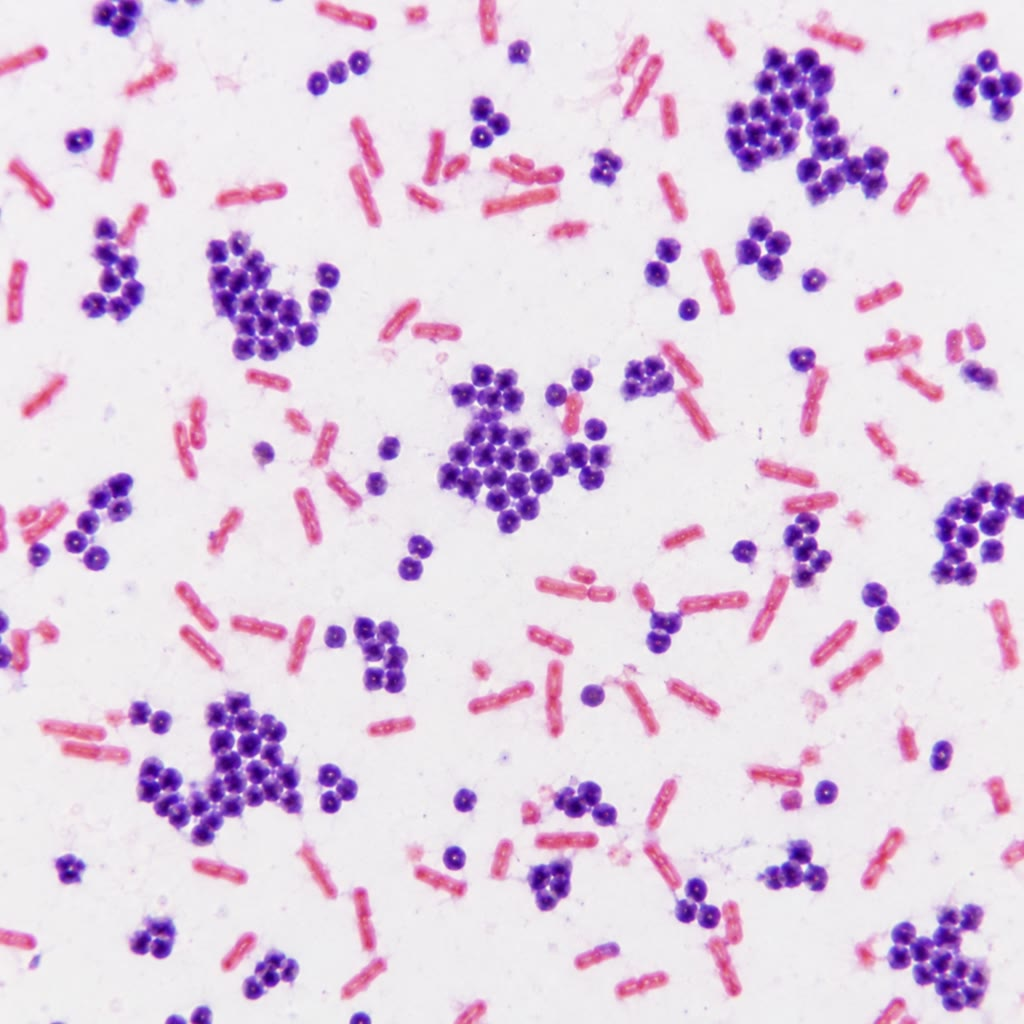
\includegraphics[width=0.36\linewidth]{images/book5/ai/b5-12-gram-stain.jpg}\hspace{0.04\linewidth}
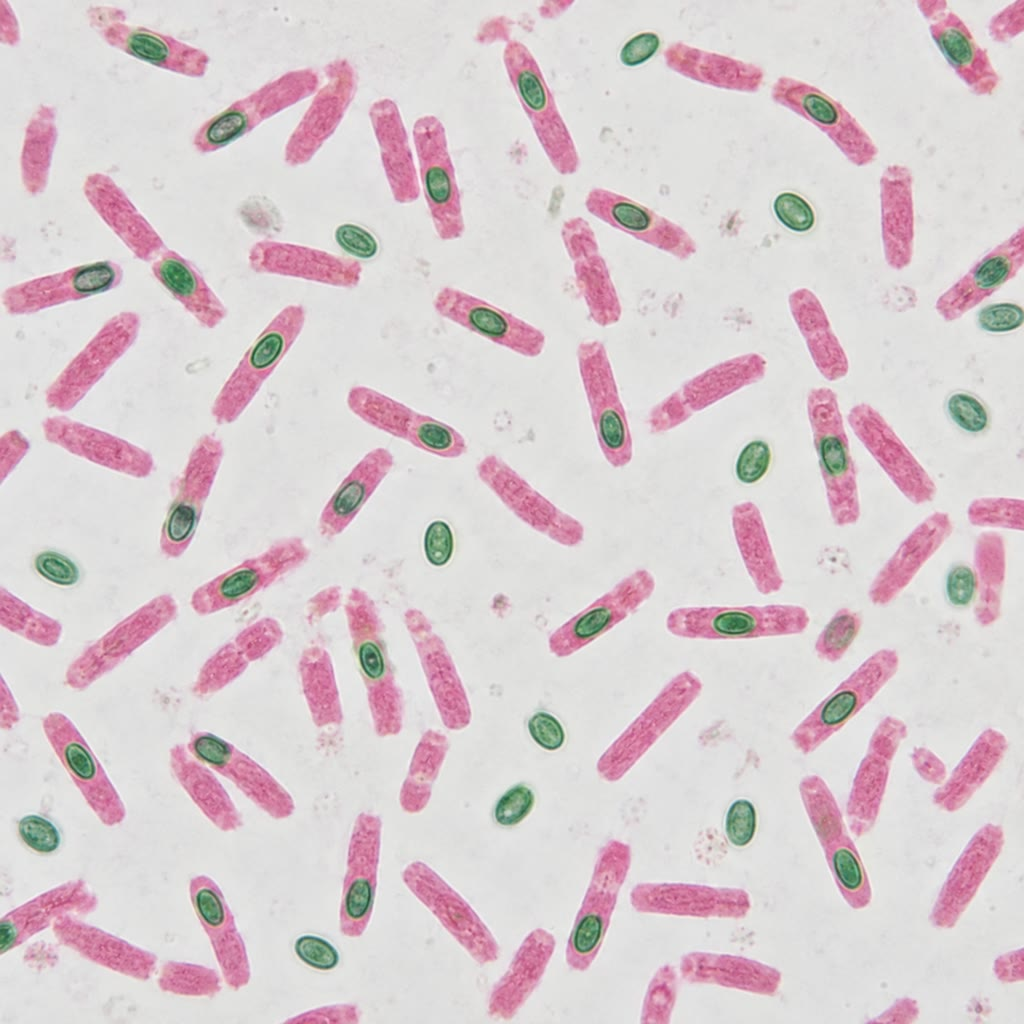
\includegraphics[width=0.36\linewidth]{images/book5/ai/b5-12-endospores.jpg}

{\small 左：\omterm{met:b3:bacteriology:gram}{革兰氏染色}——成簇的紫色\omterm{def:b3:bacteriology:envelope}{革兰氏阳性}球菌，
粉红色的\omterm{def:b3:bacteriology:envelope}{革兰氏阴性}杆菌。右：经\omterm{def:b3:bacteriology:envelope}{芽孢}染色的 \emph{Bacillus} 细胞，
\omterm{def:b3:bacteriology:envelope}{芽孢}染色后呈亮绿色的椭圆形，位于粉红色细胞内，游离的孢子
位于其旁。}
\end{omfigure}

\begin{omfigure}
\begin{tikzpicture}[every node/.style={font=\scriptsize}, >=stealth]
  % Gram-positive
  \begin{scope}
    \fill[omDef!15] (0,0) rectangle (4.5,0.4); \draw[thick, omDef] (0,0) -- (4.5,0); \draw[thick, omDef] (0,0.4) -- (4.5,0.4);
    \fill[omProp!40] (0,0.5) rectangle (4.5,2.0); \foreach \y in {0.7,0.95,1.2,1.45,1.7} \draw[omProp!80!black, thin] (0,\y) -- (4.5,\y);
    \foreach \x in {0.6,1.6,2.6,3.6} \draw[omMeth!70!black, thick] (\x,0.5) -- (\x,2.3);
    \node[below] at (2.25,-0.1) {细胞膜};
    \node[right, align=left] at (4.6,1.25) {厚肽聚糖层 \\(\qtyrange{20}{80}{nm})}; \node[right, omMeth!70!black] at (4.6,2.2) {磷壁酸};
    \node[above, font=\small\bfseries] at (2.25,2.5) {革兰氏阳性};
  \end{scope}
  % Gram-negative
  \begin{scope}[xshift=8.6cm]
    \fill[omDef!15] (0,0) rectangle (4.5,0.4); \draw[thick, omDef] (0,0) -- (4.5,0); \draw[thick, omDef] (0,0.4) -- (4.5,0.4);
    \fill[omProp!40] (0,0.75) rectangle (4.5,1.05); \draw[omProp!80!black, thin] (0,0.9) -- (4.5,0.9);
    \fill[omDef!15] (0,1.5) rectangle (4.5,1.9); \draw[thick, omDef] (0,1.5) -- (4.5,1.5); \draw[thick, omDef] (0,1.9) -- (4.5,1.9);
    \foreach \x in {0.4,0.9,1.4,1.9,2.4,2.9,3.4,3.9} \draw[omThm, thick] (\x,1.9) -- (\x,2.35);
    \draw[thick, fill=white] (2.0,1.45) rectangle (2.5,1.95); \node[below, font=\tiny] at (2.25,1.45) {孔蛋白};
    \node[below] at (2.25,-0.1) {细胞膜};
    \node[right] at (4.6,0.9) {薄肽聚糖层}; \node[right] at (4.6,1.7) {外膜}; \node[right, omThm] at (4.6,2.25) {LPS（内毒素）};
    \node[right, font=\tiny] at (4.6,1.27) {周质};
    \node[above, font=\small\bfseries] at (2.25,2.5) {革兰氏阴性};
  \end{scope}
\end{tikzpicture}

{\small 两种包膜。\omterm{def:b3:bacteriology:envelope}{革兰氏阳性}菌在膜外包裹多层
\omterm{def:b3:bacteriology:envelope}{肽聚糖}；\omterm{def:b3:bacteriology:envelope}{革兰氏阴性}菌则有一薄层\omterm{def:b3:bacteriology:envelope}{肽聚糖}和一层\omterm{def:b3:bacteriology:envelope}{外膜}，
\omterm{def:b3:bacteriology:envelope}{外膜}由\omterm{def:b3:bacteriology:envelope}{脂多糖}构成，其中嵌有孔蛋白，
可将许多\omterm{def:b3:bacteriology:antibiotics}{抗生素}挡在外面，并产生引起脓毒性休克的内毒素。}
\end{omfigure}

\section{生长}

\begin{theorem}[指数生长、莫诺定律与恒化器]\label{thm:b3:bacteriology:monod}
\index{指数生长!细菌}\index{莫诺方程}\index{恒化器}\index{稀释速率}
由 $N$ 个细胞组成的种群，以世代时间 $T$ 分裂，其增长为
$N(t) = N_{0}\,2^{t/T} = N_{0}e^{\mu t}$，比生长速率 $\mu =
\ln 2/T$。该速率随限制性营养物质 $S$ 而变，其关系由
\emph{莫诺定律}给出：
\[
\mu(S) = \mu_{\max}\,\frac{S}{K_{S} + S},
\],
饱和于 $\mu_{\max}$，并在 $S = K_{S}$ 时达到半最大值。在
\emph{\omterm{thm:b3:bacteriology:monod}{恒化器}}——一个体积为 $V$ 的容器，
向其中流入营养物浓度为 $S_{0}$ 的新鲜培养基，流速为 $F$，
培养物以相同速率流出，\omterm{thm:b3:bacteriology:monod}{稀释速率}为 $D = F/V$——
稳态时有
\[
\mu(S^{*}) = D,\qquad S^{*} = \frac{K_{S}D}{\mu_{\max} - D},\qquad
X^{*} = Y\,(S_{0} - S^{*}),
\]
其中 $X$ 为细胞密度，$Y$ 为产率（单位营养物所产生的
细胞数）。实验者通过调节泵设定生长速率；
培养物则通过调整其留下的营养物浓度作出响应。若 $D$
超过 $\mu(S_{0})$，细胞则无法跟上，并被冲出。
\end{theorem}
\begin{proof}
细胞：$\mathrm{d}X/\mathrm{d}t = \mu(S)X - DX$，即生长减去流出；
在 $X^{*} > 0$ 的稳态下，$\mu(S^{*}) = D$，反解
莫诺定律即得 $S^{*}$。营养物：$\mathrm{d}S/\mathrm{d}t = D(S_{0} -
S) - \mu(S)X/Y$，即流入减流出再减消耗；在稳态时
$\mu = D$，$D(S_{0} - S^{*}) = DX^{*}/Y$，由此得 $X^{*}$。
稳态存在的条件是 $S^{*} < S_{0}$，即 $D <
\mu(S_{0})$；超过此值时，唯一的稳态为 $X = 0$，即冲出。
稳定性：若 $X$ 高于 $X^{*}$，则消耗更多，$S$ 低于
$S^{*}$，$\mu$ 低于 $D$，$X$ 随之下降——
一个经由营养物实现的负反馈。
\end{proof}

\begin{example}[数字中的培养物]\label{ex:b3:bacteriology:numbers}
\emph{E.~coli} 在富营养培养基中，于 \qty{37}{\celsius} 培养：$T = \qty{20}{min}$，
$\mu = \qty{2.1}{h^{-1}}$。从一个细胞出发，十二小时后得到 $2^{36}$ 个细胞，
即 $7\times 10^{10}$ 个细胞，约重 \qty{70}{mg}，此时一个
\qty{100}{mL} 的烧瓶因缺氧和缺糖而停止增长；“两天内的地球
质量”相当于 $2^{144}\approx 10^{43}$ 个细胞，这一计算
只说明指数增长不可能持续。在
以葡萄糖为碳源的\omterm{thm:b3:bacteriology:monod}{恒化器}中，取 $\mu_{\max} = \qty{1.0}{h^{-1}}$，$K_{S} =
\qty{0.01}{g/L}$，$S_{0} = \qty{1}{g/L}$，每克葡萄糖可产生 $Y = \qty{0.5}{g}$ 细胞，
当\omterm{thm:b3:bacteriology:monod}{稀释速率}为 \qty{0.5}{h^{-1}} 时，葡萄糖的稳态浓度为 $S^{*}
= 0.01\times 0.5/0.5 = \qty{0.01}{g/L}$，细胞稳态浓度为 $X^{*} =
\qty{0.495}{g/L}$，细胞每 \qty{83}{min} 分裂一次，并可无限期维持。
\omterm{thm:b3:bacteriology:monod}{恒化器}可用于研究固定生长速率下的生理学，
也可在一个瓶子里进行数千代的演化实验。
\end{example}

\begin{omfigure}
\begin{tikzpicture}
\begin{axis}[
  width=6.6cm, height=5.4cm,
  axis x line=bottom, axis y line=left,
  xmin=0, xmax=14, ymin=1e6, ymax=1e10, ymode=log,
  xlabel={小时}, ylabel={每毫升细胞数},
  xlabel style={font=\small, at={(axis description cs:0.5,-0.12)}, anchor=north}, ylabel style={font=\small},
  tick label style={font=\scriptsize}, xtick={0,4,8,12},
  clip=false,
]
\addplot[very thick, omDef, domain=0:1.5, samples=2] {1e6};
\addplot[very thick, omDef, domain=1.5:7.5, samples=40] {1e6*2^((x-1.5)/0.5)};
\addplot[very thick, omDef, domain=7.5:12, samples=2] {4.1e9};
\addplot[very thick, omDef, domain=12:14, samples=10] {4.1e9*exp(-0.15*(x-12))};
\node[font=\scriptsize, anchor=south] at (axis cs:0.8,1.2e6) {延滞期};
\node[font=\scriptsize, anchor=west] at (axis cs:2.5,3e8) {指数生长期：$T = \qty{30}{min}$};
\node[font=\scriptsize, anchor=north] at (axis cs:10,3.5e9) {稳定期};
\node[font=\scriptsize, anchor=north] at (axis cs:12.8,2.2e9) {死亡期};
\end{axis}
\begin{axis}[
  at={(7.8cm,0)}, anchor=south west,
  width=6.6cm, height=5.4cm,
  axis x line=bottom, axis y line=left,
  xmin=0, xmax=0.1, ymin=0, ymax=1.1,
  xlabel={葡萄糖 $S$ (g/L)}, ylabel={$\mu$ (h$^{-1}$)},
  xlabel style={font=\small, at={(axis description cs:0.5,-0.12)}, anchor=north}, ylabel style={font=\small},
  tick label style={font=\scriptsize}, xtick={0,0.01,0.05,0.1}, xticklabels={0,$K_S$,0.05,0.1}, ytick={0,0.5,1},
  clip=false,
]
\addplot[very thick, omThm, domain=0:0.1, samples=60] {x/(0.01+x)};
\addplot[dashed, gray, domain=0:0.1, samples=2] {1};
\addplot[dashed, gray] coordinates {(0.01,0) (0.01,0.5)}; \addplot[dashed, gray] coordinates {(0,0.5) (0.01,0.5)};
\node[font=\scriptsize, omThm, anchor=north west] at (axis cs:0.045,0.6) {莫诺：$\mu = \mu_{\max}S/(K_{S}+S)$};
\node[font=\scriptsize, gray, anchor=south east] at (axis cs:0.1,1.01) {$\mu_{\max}$};
\end{axis}
\end{tikzpicture}

{\small 左图：分批培养——酶诱导期间的\omterm{def:b3:bacteriology:phases}{延滞期}，
指数生长、营养物耗尽后的\omterm{def:b3:bacteriology:phases}{稳定期}，以及
缓慢死亡。右图：莫诺定律，即生长速率与限制性营养物浓度的关系，
其中 $K_{S}$ 为半最大生长速率对应的浓度。}
\end{omfigure}

\begin{definition}[时期与状态]\label{def:b3:bacteriology:phases}
\index{延滞期}\index{稳定期}\index{芽孢形成}\index{σ 因子}
在新鲜烧瓶中（称为\emph{分批培养}），细胞起初停顿——即
\emph{延滞期}，此时细胞诱导合成新培养基所需的酶，
随后呈指数生长，直到某种营养物耗尽或
废物积累时停止增长，即\emph{稳定期}，此时细胞
变小，加厚被膜，使拟核凝缩于
保护性蛋白周围，并通过替代性
σ 因子 RpoS 开启应激基因，可存活数月；随后进入死亡期，
其间大多数细胞裂解，少数细胞依靠残骸存活。某些物种
以发育程序应对饥饿：\emph{Bacillus
subtilis}进行不对称分裂，较大的细胞包裹较小的细胞，
并围绕其形成\omterm{def:b3:bacteriology:envelope}{芽孢}，该过程持续八小时，
受一系列\emph{σ 因子}级联调控——σ 因子即
引导 RNA 聚合酶识别某一组启动子的亚基——该级联
在两个区室之间交替进行，是细菌分化的首例，
也是细胞间借细胞壁传递信号的首例。
\end{definition}

\section{相互感知}

\begin{definition}[群体感应]\label{def:b3:bacteriology:quorum}
\index{群体感应}\index{自诱导物}\index{双组分系统}
细菌通过\emph{群体感应}感知自身的密度：每个细胞
以恒定速率分泌一种小信号分子，即\emph{自诱导物}——\omterm{def:b3:bacteriology:envelope}{革兰氏阴性}菌中为
酰化高丝氨酸内酯，\omterm{def:b3:bacteriology:envelope}{革兰氏阳性}菌中为短肽——
培养基中的浓度随
细胞数量增加而升高，超过阈值时便与受体结合，
开启一组基因，其中包括
自诱导物本身的合成酶（由此得名）。受此调控的基因正是那些
只在群体中才有益的基因：\emph{Vibrio fischeri} 的发光，
\emph{Staphylococcus aureus} 与
\emph{Pseudomonas aeruginosa} 的毒力因子、生物膜基质、
摄取 DNA 的感受态，以及杀伤邻近细胞。大多数细菌的感知
依靠\emph{双组分系统}完成：膜上的组氨酸激酶
感知刺激，并使胞质内的应答调节蛋白磷酸化，
后者结合 DNA——一个细胞拥有数十种这样的系统，分别感知磷酸盐、渗透浓度、
氧气以及其他物种的自诱导物。
\end{definition}

\begin{proof}[证据]
尼尔森、普拉特和黑斯廷斯（1970）培养了发光的海洋细菌
 \emph{Vibrio fischeri}，从稀释的接种物开始培养，发现细胞
不发光，直到密度达到约 $10^{7}$ 个
每毫升时才同时全部发光；将已在高密度培养物中生长过的培养基
灭菌后加入稀释的培养物中，立即使其发光。
这说明细胞感知的是一种分泌物质，而非时间或
营养物。该物质经鉴定为一种酰化高丝氨酸内酯
（埃伯哈德，1981）；相关基因——\emph{luxI} 编码合成酶，
\emph{luxR} 编码受体，以及它们所调控的荧光素酶操纵子——
被克隆到 \emph{E.~coli} 中，使其在密度高时发光。在
容纳该细菌的鱿鱼体内，细菌密度达 $10^{10}$ 个每毫升，
光器官发光；而在海洋中，由于细菌稀少，它们
保持暗淡，从而省下这一代价。
\end{proof}

\begin{proposition}[密度阈值]\label{prop:b3:bacteriology:threshold}
\index{群体感应!阈值}
设 $N$ 个细胞位于体积 $V$ 中，各细胞以速率
$p$ 个分子每秒分泌\omterm{def:b3:bacteriology:quorum}{自诱导物}，且该分子以一级速率
$k$ 消失（降解或稀释）。浓度趋于
$A^{*} = pN/(kV)$，与细胞密度 $N/V$ 成正比，
时间常数为 $1/k$；当 $A^{*}$ 达到其
阈值 $A_{\text{阈}}$ 时受体开启，即密度为
\[
\left(\frac{N}{V}\right)_{\text{阈}} = \frac{k\,A_{\text{阈}}}{p}.
\]
。在封闭空间中——鱿鱼的光器官、脓肿、
肺部的黏液——$k$ 很小，因为信号不会被带走，所以
达到阈值密度所需的细胞较少；在开阔水体中，
则永远达不到。因此，细胞测量的不是
自身的数量，而是单位体积内所共享的数量，这正是
任何协同行为的关键；\omterm{def:b3:bacteriology:quorum}{自诱导物}对其自身合成酶的正反馈
使开关变得陡峭：一旦少数细胞越过阈值，
它们额外的产出便推动其余细胞越过阈值。
\end{proposition}
\begin{proof}
$\mathrm{d}A/\mathrm{d}t = pN/V - kA$ 的稳态为 $A^{*} =
pN/(kV)$，并以 $e^{-kt}$ 的形式趋于该稳态。令 $A^{*} = A_{\text{阈}}$
解出 $N/V$，即得阈值密度。
\end{proof}

\begin{omfigure}
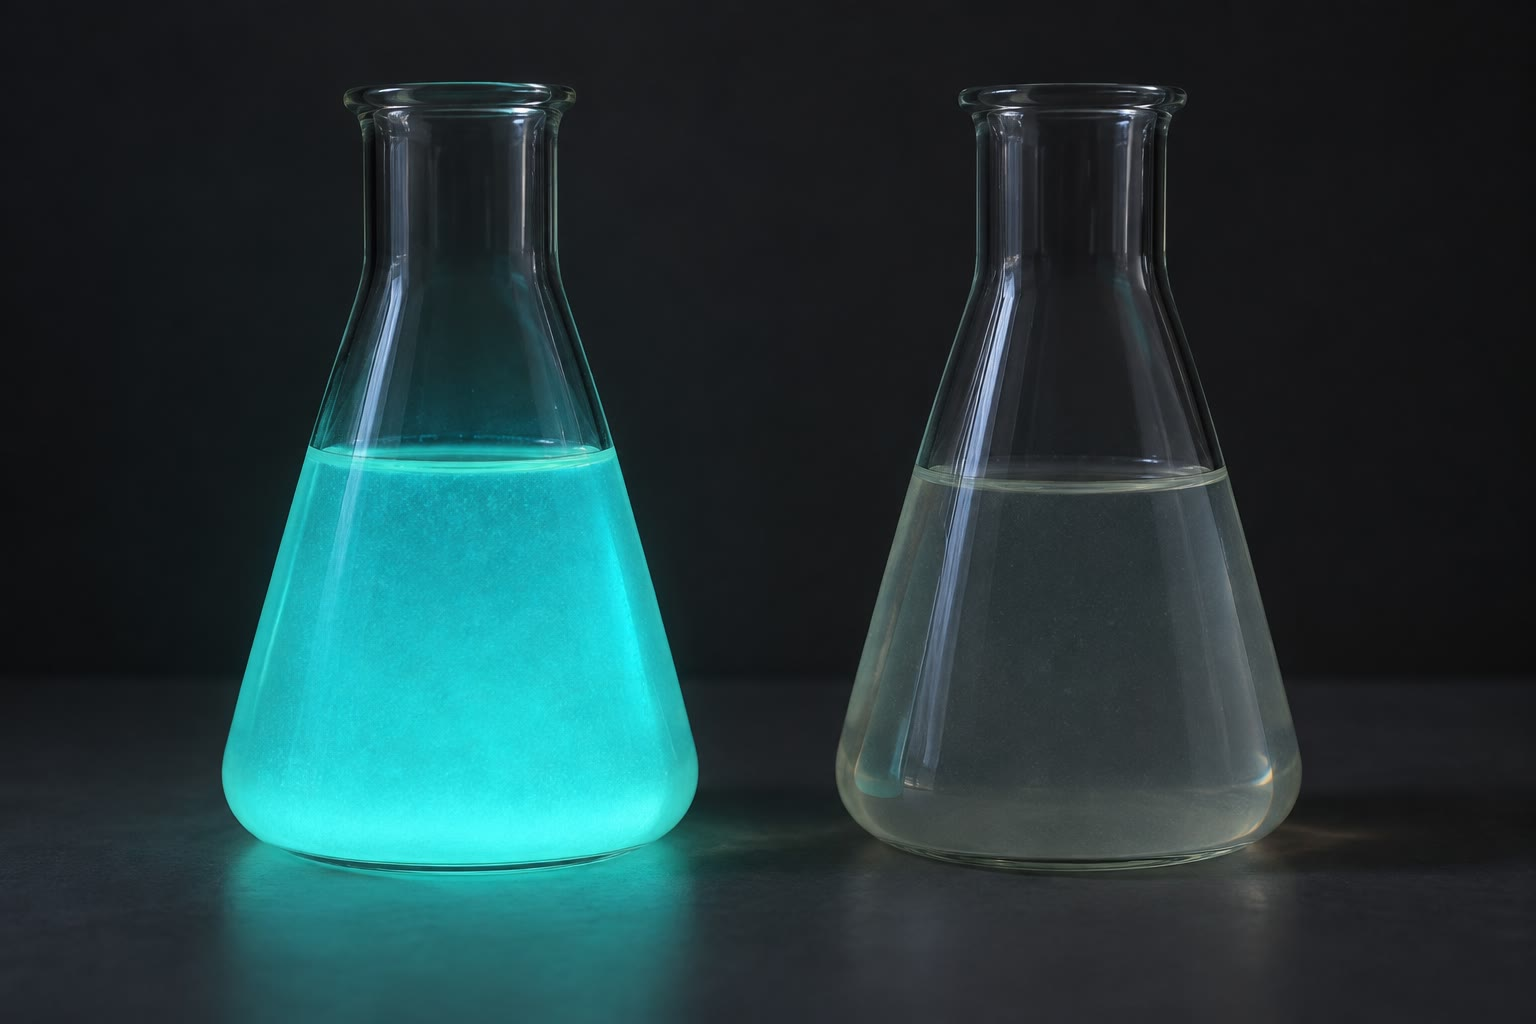
\includegraphics[width=0.46\linewidth]{images/book5/ai/b5-12-quorum-glow.jpg}\hspace{0.04\linewidth}
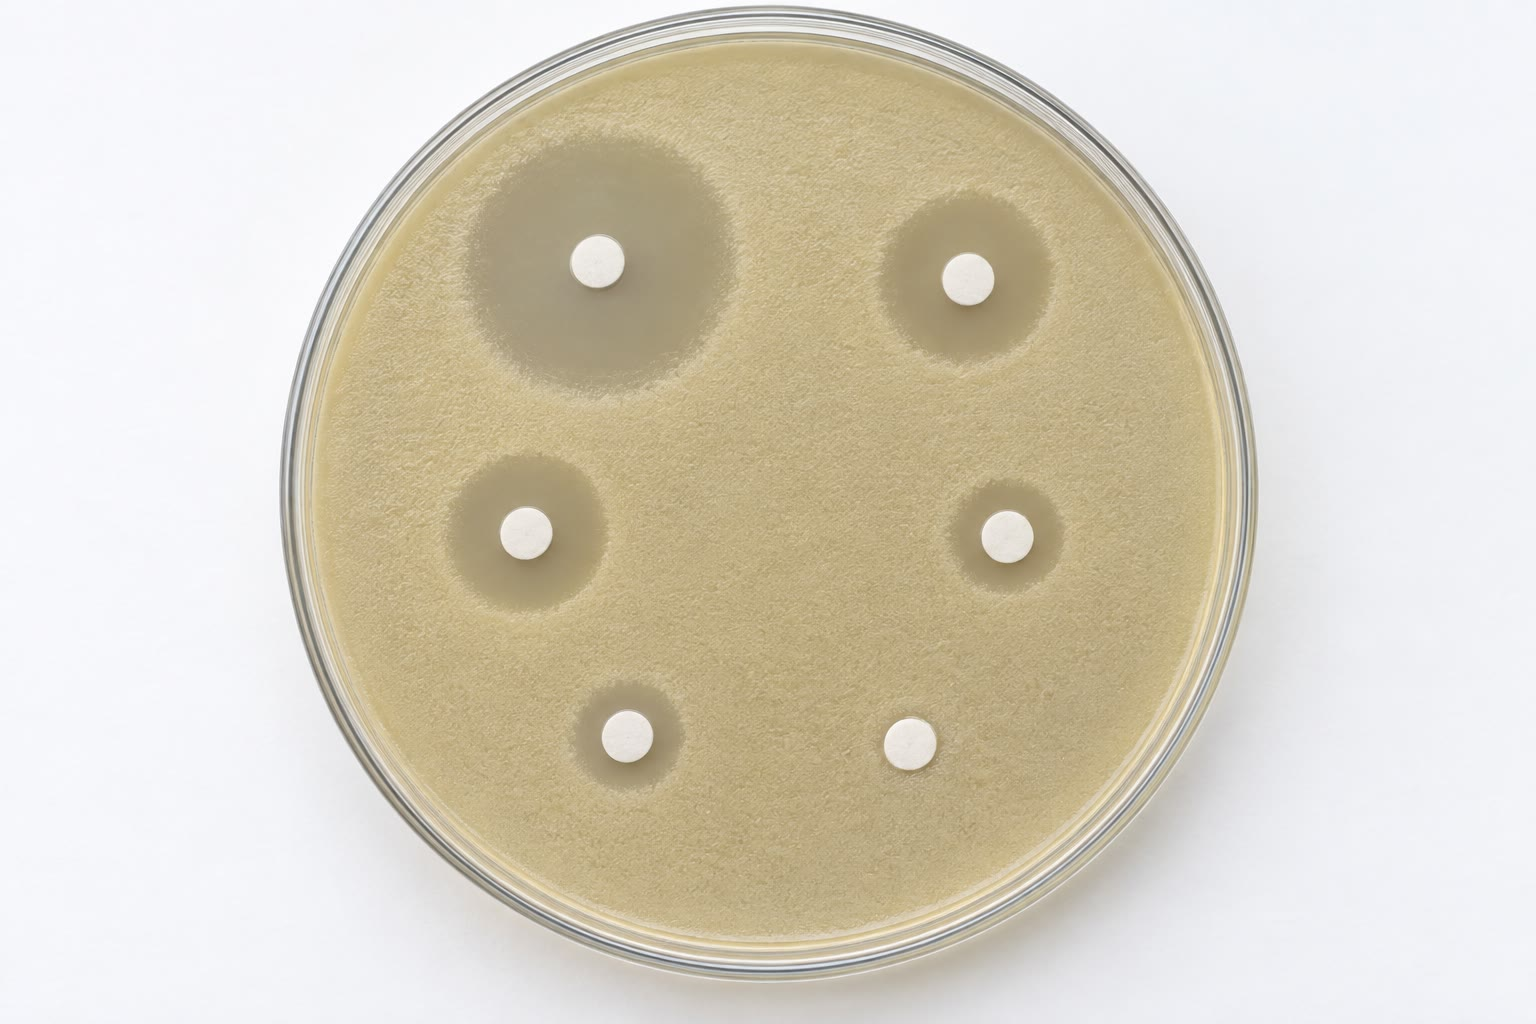
\includegraphics[width=0.46\linewidth]{images/book5/ai/b5-12-antibiotic-disks.jpg}

{\small 左：致密的 \emph{Vibrio fischeri} 培养物发光，旁边是
稀疏而不发光的培养物——同样的细胞，分别处于
其\omterm{def:b3:bacteriology:quorum}{群体感应}阈值之上和之下。右：纸片扩散试验；每个透明抑菌圈的直径
度量该细菌对该纸片上\omterm{def:b3:bacteriology:antibiotics}{抗生素}的敏感程度，
而无抑菌圈的纸片则表明存在抗性。}
\end{omfigure}

\section{基因的流动}

\begin{definition}[基因水平转移]\label{def:b3:bacteriology:hgt}
\index{转化}\index{转导}\index{接合}\index{质粒!抗性}\index{移动遗传元件}\index{泛基因组}
细菌以克隆方式繁殖，但通过三条途径交换基因。
\emph{转化}：感受态细胞从环境中摄取
裸露的 DNA——格里菲思的肺炎链球菌正是借此获得其荚膜，
埃弗里于 1944 年证明转化因子是 DNA。
\emph{转导}：噬菌体包装一段宿主 DNA，
并将其注入下一个宿主（见\cref{ch:b3:virology}）。
\emph{接合}：\omterm{def:b3:genetic-engineering:tools}{质粒}经由菌毛和
交配桥，从携带它的供体菌\omterm{def:b3:cancer-biology:hallmarks}{转移}至受体菌，
此过程由莱德伯格和塔特姆于 1946 年以营养缺陷型的 \emph{E.~coli} 菌株证明，
这些菌株只有混合后才产生原养型重组体。接合型\omterm{def:b3:genetic-engineering:tools}{质粒}携带
自身的\omterm{def:b3:cancer-biology:hallmarks}{转移}基因；许多\omterm{def:b3:genetic-engineering:tools}{质粒}还携带抗性基因，这些基因
常聚集于\emph{整合子}中，两侧带有转座子，
因此，一次交配即可同时\omterm{def:b3:cancer-biology:hallmarks}{转移}对五种\omterm{def:b3:bacteriology:antibiotics}{抗生素}的抗性，
且可跨越物种。其结果是，一个细菌物种既有
所有菌株共有的核心基因组，也有
各不相同的附加基因组——即\emph{泛基因组}：两株 \emph{E.~coli} 菌株
的基因可相差五分之一，而致病菌株与
无害菌株之间的差异主要在于所获得的毒力基因岛。本科二年级分册突变一章中的基因
主要经突变产生；本章的基因则
大多是“送上门来”的。
\end{definition}

\begin{omfigure}
\begin{tikzpicture}[every node/.style={font=\scriptsize}, >=stealth]
  % transformation
  \begin{scope}
    \draw[thick, fill=omDef!15] (0,0) ellipse (1.0 and 0.55);
    \draw[omThm, very thick] (-1.9,0.6) .. controls (-1.5,0.8) .. (-1.2,0.5); \draw[->, omThm, thick] (-1.2,0.5) -- (-0.7,0.25);
    \node[below, align=center] at (0,-0.7) {转化：\\裸露的 DNA 被 \\感受态细胞摄取};
  \end{scope}
  % transduction
  \begin{scope}[xshift=4.6cm]
    \draw[thick, fill=omDef!15] (0,0) ellipse (1.0 and 0.55);
    \draw[thick, fill=omProp!40] (-1.3,1.0) -- (-1.0,1.3) -- (-0.7,1.0) -- (-1.0,0.7) -- cycle; \draw[thick] (-1.0,0.7) -- (-0.9,0.35);
    \draw[omThm, very thick] (-1.1,1.15) -- (-0.9,0.85);
    \node[below, align=center] at (0,-0.7) {转导：\\噬菌体携带一段 \\上一宿主的 DNA};
  \end{scope}
  % conjugation
  \begin{scope}[xshift=9.6cm]
    \draw[thick, fill=omDef!15] (-1.3,0) ellipse (0.9 and 0.5); \draw[thick, fill=omDef!15] (1.3,0) ellipse (0.9 and 0.5);
    \draw[very thick, omMeth!70!black] (-0.4,0) -- (0.4,0);
    \draw[omThm, very thick] (-1.5,0) circle (0.25); \draw[->, omThm, thick] (-1.25,0) -- (1.0,0);
    \node[below, align=center] at (0,-0.7) {接合：\\质粒穿过 \\交配桥};
  \end{scope}
\end{tikzpicture}

{\small 水平\omterm{def:b3:cancer-biology:hallmarks}{转移}的三条途径。抗性、毒力和代谢基因
在细胞之间——乃至物种之间——流动，速度远超
突变产生它们的速度。}
\end{omfigure}

\begin{proof}[证据]
科赫（1876--1884）确立了：某一特定细菌导致某一特定
疾病。他从患病动物体内分离出 \emph{Bacillus anthracis}，
并在固体培养基上进行纯培养（琼脂平板和
单菌落均为他实验室的发明），并证明该培养物
可使健康动物患炭疽，且能从其体内重新分离出该菌——
这即至今仍用以界定病原体的科赫法则——并进而
研究结核杆菌与霍乱弧菌。1928 年，弗莱明
注意到，污染葡萄球菌平板的霉菌已
在其周围形成一圈透明区；这种物质即青霉素，经纯化后
由弗洛里和钱恩于 1940--1941 年证明可治愈感染，
十年之内，携带能破坏青霉素之酶的耐药葡萄球菌
在医院中已相当普遍——这是弗莱明本人在
其诺贝尔奖演讲中所发出的警告。
\end{proof}

\begin{omfigure}
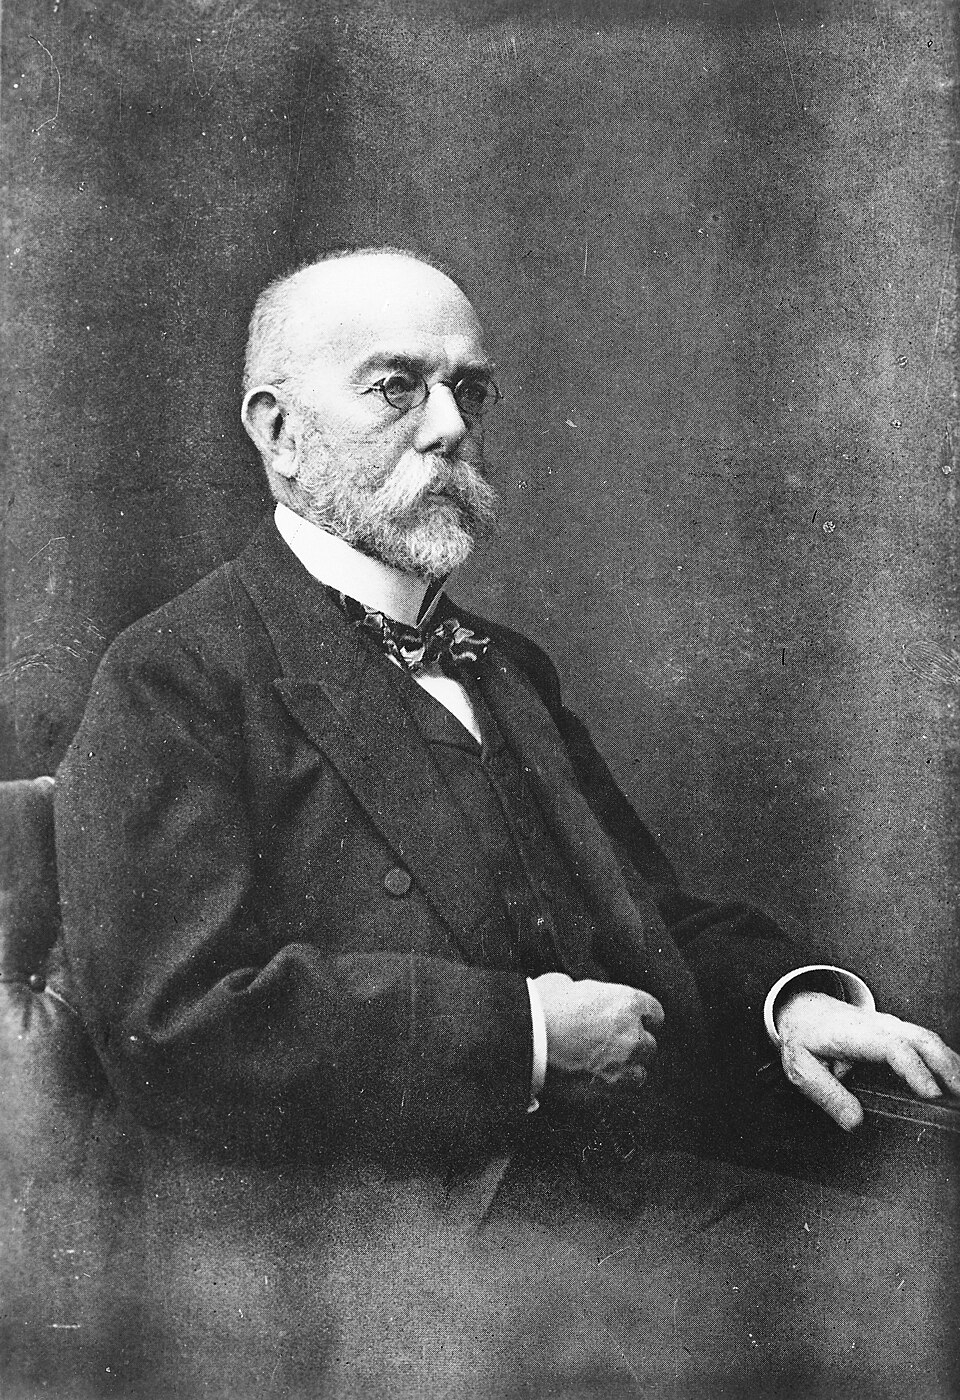
\includegraphics[width=0.30\linewidth]{images/book5/koch.jpg}\hspace{0.04\linewidth}
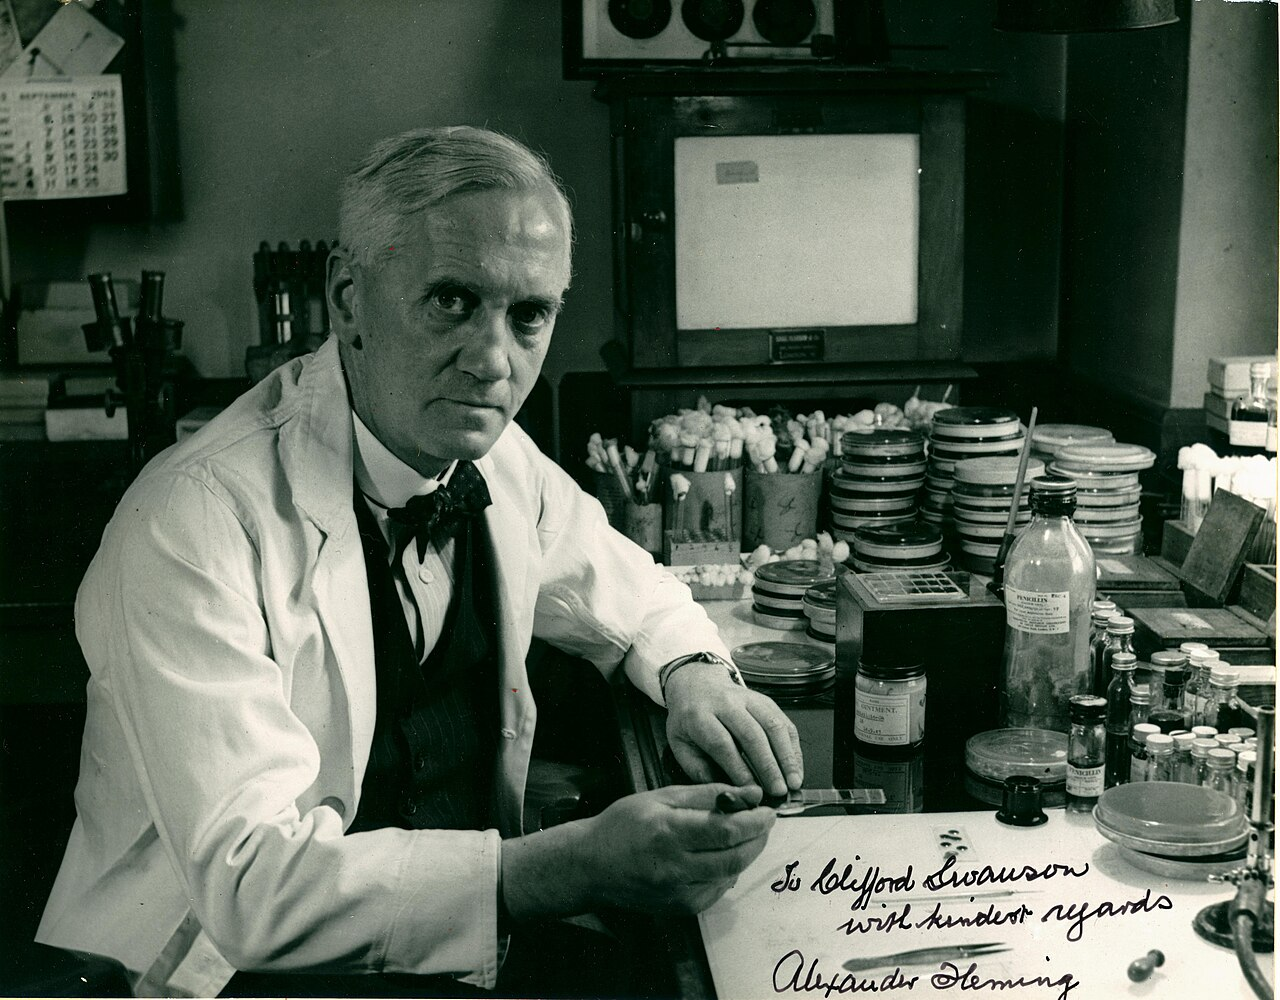
\includegraphics[width=0.56\linewidth]{images/book5/fleming.jpg}

{\small 罗伯特·科赫，证明了特定细菌引起特定疾病，
并发明了培养这些细菌的方法（Wellcome
Collection, CC~BY~4.0）。右图：亚历山大·弗莱明在其实验室中，
与培养皿中的霉菌合影，该霉菌的产物即青霉素（美国海军
档案，公有领域）。}
\end{omfigure}

\section{抗生素与抗性}

\begin{definition}[抗生素]\label{def:b3:bacteriology:antibiotics}
\index{抗生素}\index{β-内酰胺类}\index{选择性毒性}\index{最低抑菌浓度}
\emph{抗生素}是一类分子，能在对宿主无害的浓度下杀死细菌或抑制其
生长，通过作用于宿主所无或形式不同的靶点，这种性质称为
\emph{选择性
毒性}。靶点不多。细胞壁方面：\emph{$\beta$-内酰胺类}
（青霉素、头孢菌素、碳青霉烯类）模拟\omterm{def:b3:bacteriology:envelope}{肽聚糖}肽段的末端
D-Ala-D-Ala 序列，并使催化\omterm{def:b3:bacteriology:envelope}{肽聚糖}交联的酶发生酰化，
使生长中的细胞壁变弱，细胞在
自身膨压下破裂；万古霉素则直接结合 D-Ala-D-Ala 本身。
核糖体（其细菌形式不同于真核形式）：氨基糖苷类
（作用于小亚基，导致错读）、四环素类（阻断 tRNA
进入）、大环内酯类和氯霉素（作用于大亚基的出口
通道与肽基\omterm{def:b3:cancer-biology:hallmarks}{转移}酶）。DNA 旋转酶与拓扑异构酶~IV：
喹诺酮类。RNA 聚合酶：利福平。叶酸合成，此为
动物所不具备：磺胺类与甲氧苄啶。细胞膜：多黏菌素类，
属最后的手段。\emph{最低抑菌浓度}
（MIC）是能阻止某菌株出现可见
生长的最低药物浓度；当某菌株的 MIC 超过
药物在患者体内所能达到的浓度时，该菌株即称为耐药。
\end{definition}

\begin{method}[测定敏感性]\label{met:b3:bacteriology:mic}
\index{纸片扩散法}\index{肉汤稀释法}
两种方法。\emph{\omterm{met:b3:bacteriology:mic}{肉汤稀释法}}：取定量细胞
（每毫升约 $5\times 10^{5}$ 个）接种到一排试管或孔板中，
各管中含有按二倍梯度递增的\omterm{def:b3:bacteriology:antibiotics}{抗生素}，过夜孵育，
读取第一个澄清的孔：该浓度即为 MIC。\emph{\omterm{met:b3:bacteriology:mic}{纸片
扩散法}}：将菌株涂布于琼脂平板上，放置
载有已知量多种\omterm{def:b3:bacteriology:antibiotics}{抗生素}的纸片，孵育；药物
向外扩散，浓度随距离下降，生长
被抑制的范围直至浓度等于 MIC 的半径处为止，
因此抑菌圈的直径——对照校准
表读取——即可得到同一平板上每张纸片的敏感性。两种
方法均需一天；对基因组测序以检测已知耐药基因及
突变同样需一天，且正逐步取代它们。
\end{method}

\begin{definition}[抗性]\label{def:b3:bacteriology:resistance}
\index{抗生素抗性}\index{β-内酰胺酶}\index{外排泵}\index{MRSA}
细菌抵抗\omterm{def:b3:bacteriology:antibiotics}{抗生素}的方式有五种。其一是破坏
药物：\emph{$\beta$-内酰胺酶}水解 $\beta$-内酰胺环，
而超广谱及碳青霉烯酶变体如今能破坏
最新的药物。其二是改变靶点：药物所结合的核糖体蛋白或
旋转酶发生突变，或在 MRSA（耐甲氧西林
\emph{Staphylococcus aureus}）中获得一个编码交联酶的基因，
$\beta$-内酰胺类不能与之结合；万古霉素耐药则是
用 D-乳酸取代末端的 D-Ala，药物不再能识别。
其三是借\emph{外排泵}把药物泵出，这类泵常具广谱
专一性。其四是阻止药物进入，方法是丢失一种孔蛋白。或
者以替代酶绕过被阻断的步骤。靶点突变
随机出现于患者体内，每次分裂的突变率为 $10^{-8}$ 至 $10^{-6}$，
并在治疗期间被选择。酶与泵大多
经\omterm{def:b3:genetic-engineering:tools}{质粒}从土壤和肠道细菌的巨大储库中获得，
这些酶与泵在储库中历经漫长岁月，针对真菌和其他细菌所产生的
\omterm{def:b3:bacteriology:antibiotics}{抗生素}而演化。持留菌即休眠细胞，它们能在
药物作用下存活而无遗传抗性——这类细胞可解释
治疗本应奏效之后仍发生的复发。
\end{definition}

\begin{proposition}[为何抗性不可避免，联合用药是解决之道]\label{prop:b3:bacteriology:selection}
\index{抗性!选择}\index{联合疗法!抗生素}
若以一种药物治疗含 $10^{9}$ 个细胞的感染，该药物所针对的
抗性突变以每次分裂 $10^{-8}$ 的频率出现，该感染中已含有
约十个耐药细胞；药物杀死其余细胞，这十个细胞
便会占据优势——与\cref{ch:b3:cancer-biology}中的计算完全一致，因为一个
细菌种群与\omterm{def:b3:cancer-biology:hallmarks}{肿瘤}都是处于
选择作用下演化的克隆。两种靶点独立的药物所面对的
双重抗性细胞，其频率为每次分裂 $10^{-16}$，十亿个细胞中也不会存在。
这正是结核病的情形：其病灶中含有 $10^{8}$--$10^{9}$ 个
杆菌，自 20 世纪 50 年代起便同时使用三到四种药物治疗，
而单药治疗在数月内即产生抗性；这也是
为何无论在患者身上还是在饲养场中使用\omterm{def:b3:bacteriology:antibiotics}{抗生素}，都会在某处
选出抗性，以及新\omterm{def:b3:bacteriology:antibiotics}{抗生素}的研发速率（自 1960 年代以来，
尚无针对\omterm{def:b3:bacteriology:envelope}{革兰氏阴性}菌的新类别）——这一速率即
计算损失所依据的标尺。应对之策与任何进化竞争一样：
少用药、联合用药、完成疗程，使
部分抗性细胞无法存活并繁殖，并寻找新的
靶点。
\end{proposition}

\begin{example}[突变体选择窗口]\label{ex:b3:bacteriology:window}
某菌株的 MIC 为 \qty{1}{mg/L}；其一步突变所得的抗性突变体，
频率为 $10^{7}$ 分之一，其 MIC 为 \qty{8}{mg/L}。一个能将药物浓度维持在
\qty{4}{mg/L} 的剂量可杀死野生型，使突变体
无竞争地生长：介于野生型与
突变体之间的浓度范围即为\emph{突变体选择
窗口}，处于其中的治疗会培育抗性。
剂量高于 \qty{8}{mg/L} 则两者皆被杀死；若剂量过低，或
疗程在患者感觉好转、药物浓度正穿越该窗口时中止，
便是造成耐药群体的方式。同一逻辑也决定了结核病的治疗方案：
六个月，四种药物，剂量
均高于每一单步突变体的 MIC。
\end{example}

\begin{omfigure}
\begin{tikzpicture}
\begin{axis}[
  width=0.7\linewidth, height=5.6cm,
  axis x line=bottom, axis y line=left,
  xmin=0, xmax=24, ymin=0.25, ymax=32, ymode=log,
  xlabel={给药后小时数}, ylabel={血浆药物浓度 (mg/L)},
  xlabel style={font=\small, at={(axis description cs:0.5,-0.12)}, anchor=north}, ylabel style={font=\small},
  tick label style={font=\small}, xtick={0,6,12,18,24}, ytick={0.5,1,2,4,8,16}, yticklabels={0.5,1,2,4,8,16},
  clip=false,
]
\fill[omThm!15] (axis cs:0,1) rectangle (axis cs:24,8);
\addplot[very thick, omDef, domain=0:24, samples=60] {16*exp(-0.15*x)};
\addplot[dashed, gray, domain=0:24, samples=2] {1}; \addplot[dashed, gray, domain=0:24, samples=2] {8};
\node[font=\scriptsize, gray, anchor=south west] at (axis cs:0.3,1.05) {野生型的 MIC};
\node[font=\scriptsize, gray, anchor=south east] at (axis cs:23.7,8.4) {一步突变体的 MIC};
\node[font=\scriptsize, omThm!70!black, anchor=west] at (axis cs:13,3.5) {突变体选择窗口};
\node[font=\scriptsize, omDef, anchor=south west] at (axis cs:2,13) {给药后的血浆药物浓度};
\end{axis}
\end{tikzpicture}

{\small 突变体选择窗口。药物浓度高于突变体的 MIC 时，全部细菌都会被杀死；
介于两个 MIC 之间（阴影部分）时，它杀死野生型，却选择出突变体。
剂量若使药物浓度在该窗口内持续数小时，
或疗程提前终止，都会促使耐药性产生。}
\end{omfigure}

\begin{remark}[大多数细菌并非病原体]\label{rem:b3:bacteriology:most}
本章临床相关的细菌只是极少数。在估计约 100 万个物种中，
仅几百种会引起人类疾病；其余细菌参与氮、硫和碳的循环（见本科二年级分册），
固定豆科植物的氮，
分解反刍动物体内的纤维素，
并构成\cref{ch:b3:microbiomes}中的微生物组。\omterm{def:b3:bacteriology:antibiotics}{抗生素}治疗造成的
微生物组损失，是每个疗程都要付出的代价。
\omterm{def:b3:bacteriology:antibiotics}{抗生素}本身就是这些细菌的分子——
它们是在医院出现之前，于土壤细菌与真菌之间演化出的武器与信号——
大多数耐药基因也是如此。
\end{remark}

\section{练习}

\begin{exercise}[$\star$]\label{exo:b3:bacteriology:1}
描述\omterm{def:b3:bacteriology:envelope}{革兰氏阳性}菌与\omterm{def:b3:bacteriology:envelope}{革兰氏阴性}菌的包膜结构，
并说明\omterm{met:b3:bacteriology:gram}{革兰氏染色}为何能将二者区分开。
\end{exercise}

\begin{exercise}[$\star$]\label{exo:b3:bacteriology:2}
某培养物中细胞浓度为 $10^{3}$ 个每毫升，经指数生长后达到 $10^{9}$ 个每毫升，
所需时间为 \qty{8}{h}。求世代数、
世代时间以及 $\mu$。
\end{exercise}

\begin{exercise}[$\star$]\label{exo:b3:bacteriology:3}
写出水平基因\omterm{def:b3:cancer-biology:hallmarks}{转移}的三种途径，
并给出分别证明各途径的经典实验。
\end{exercise}

\begin{exercise}[$\star$]\label{exo:b3:bacteriology:4}
给出青霉素、链霉素、环丙沙星和利福平的作用靶点，
并说明每种药物为何具有\omterm{def:b3:bacteriology:antibiotics}{选择性毒性}。
\end{exercise}

\begin{exercise}[$\star\star$]\label{exo:b3:bacteriology:5}
\omterm{thm:b3:bacteriology:monod}{恒化器}中 $\mu_{\max} = \qty{0.8}{h^{-1}}$，$K_{S} =
\qty{0.02}{g/L}$，$S_{0} = \qty{2}{g/L}$，$Y = 0.4$。求 $S^{*}$ 与
$X^{*}$，分别对应 $D = 0.2$、$0.6$ 和 $0.79$ h$^{-1}$，
以及开始发生洗出的\omterm{thm:b3:bacteriology:monod}{稀释速率}。
\end{exercise}

\begin{exercise}[$\star\star$]\label{exo:b3:bacteriology:6}
利用\cref{prop:b3:bacteriology:threshold}，比较鱿鱼发光器（$k =
\qty{0.01}{h^{-1}}$）与流动海水（$k = \qty{10}{h^{-1}}$）中\omterm{def:b3:bacteriology:quorum}{群体感应}的阈值密度，
取 $p = 100$ 个分子每细胞每小时，
$A_{\text{阈}} =
\qty{10}{nmol/L}$（$6\times 10^{12}$ 个分子每升）。
\end{exercise}

\begin{exercise}[$\star\star$]\label{exo:b3:bacteriology:7}
纸片扩散平板上三种药物的抑菌圈直径分别为 $25$、$12$ 和 \qty{0}{mm}。
逐一解释这些结果，
并说明为何抑菌圈直径可以换算为 MIC。
\end{exercise}

\begin{exercise}[$\star\star$]\label{exo:b3:bacteriology:8}
解释一次\omterm{def:b3:bacteriology:hgt}{接合}事件如何使敏感的\emph{Klebsiella}
对五种\omterm{def:b3:bacteriology:antibiotics}{抗生素}同时产生耐药性，
并说明耐药基因为何常常共同位于\omterm{def:b3:genetic-engineering:tools}{质粒}上。
\end{exercise}

\begin{exercise}[$\star\star$]\label{exo:b3:bacteriology:9}
某患者体内有 $10^{9}$ 个细菌，服用一种药物后，每次分裂产生耐药性的概率为 $10^{-7}$。
计算开始时预期的耐药细胞数；
再计算使用两种独立药物时的情况。
持留菌为何是另一类问题？
\end{exercise}

\begin{exercise}[$\star\star\star$]\label{exo:b3:bacteriology:10}
证明\omterm{thm:b3:bacteriology:monod}{恒化器}的稳态是稳定的：使 $X$ 略微高于 $X^{*}$，
并跟踪 $\mathrm{d}S/\mathrm{d}t$ 与 $\mathrm{d}X/\mathrm{d}t$ 的符号。
然后解释为何在\omterm{thm:b3:bacteriology:monod}{恒化器}中，两个竞争同一种营养物质的物种
在稳态下不能共存，
并判断在给定的 $D$ 下哪一个物种获胜。
\end{exercise}

\begin{exercise}[$\star\star\star$]\label{exo:b3:bacteriology:11}
\omterm{def:b3:bacteriology:quorum}{自诱导物}可诱导其自身合成酶。修改\cref{prop:b3:bacteriology:threshold}中的模型，
使 $p$ 由 $p_{0}$ 跃升至 $p_{1} \gg p_{0}$，当 $A > A_{\text{阈}}$ 时，
并证明在一定密度范围内系统可以存在两个稳定状态（\omterm{thm:b3:cell-cycle-apoptosis:oscillator}{滞后现象}）：
已经开启的种群在该密度下仍保持开启，
而同样密度下未经历开启的种群则处于关闭状态。
这种性质在生物学上有何用途？
\end{exercise}

\begin{exercise}[$\star\star\star$]\label{exo:b3:bacteriology:12}
解释突变体选择窗口，并利用它论证以下各项的利弊：
(a) 短疗程高剂量；(b) 长疗程低剂量；
(c) 症状消失即停药；(d) 联合用药。
\end{exercise}

\section{问题：恒化器与临床}

\begin{problem}[{周末问题——在烧瓶中培养并置于恒化器中的一种发光细菌，计数至其群体感应阈值，
以及依据耐药性算术治疗的一次感染，
末尾讨论恒化器中的细胞、
光开始发出时的密度，
以及双药疗程遇到耐药细胞的概率}]
\label{pb:b3:bacteriology:1}
数据：\emph{E.~coli} 于 \qty{37}{\celsius}，$T = \qty{20}{min}$；一个细胞重 \qty{1}{pg}。
\omterm{thm:b3:bacteriology:monod}{恒化器}：$V = \qty{1}{L}$，$F = \qty{0.5}{L/h}$，$\mu_{\max} = \qty{1.0}{h^{-1}}$，
$K_{S} = \qty{0.01}{g/L}$，$S_{0} =
\qty{2}{g/L}$ 葡萄糖，$Y = 0.5$。\emph{Vibrio}：每细胞每小时
$p = 500$ 个\omterm{def:b3:bacteriology:quorum}{自诱导物}分子，$A_{\text{阈}} = 6\times 10^{12}$
个分子每升（\qty{10}{nmol/L}），光器官中 $k = \qty{0.05}{h^{-1}}$。
感染：$10^{9}$ 个细胞；对药物 A 的耐药性为每次分裂 $10^{-8}$，对药物 B 为 $10^{-7}$；
野生型对 A 的 MIC 为 \qty{1}{mg/L}，一步突变体为 \qty{8}{mg/L}；
一次给药使药物浓度达到 \qty{16}{mg/L}，
并以半衰期 \qty{4}{h} 下降。

\medskip
\noindent\textbf{第一部分——烧瓶。}
\begin{enumerate}
  \item 在 \qty{100}{mL} 培养液中有一个细胞。经过
        \qty{6}{h} 指数生长后，细胞数是多少？每毫升的密度是多少？
  \item 培养液每毫升至多支持 $2\times 10^{9}$ 个细胞。生长何时
        停止？培养物中细胞的质量是多少？
  \item 由一个细胞繁衍的后代，需要多久才能达到
        地球的质量（$6\times 10^{27}$ 克）？请加以评述。
  \item \omterm{def:b3:bacteriology:phases}{稳定期}的细胞接种到新鲜培养基中时，\omterm{def:b3:bacteriology:phases}{延滞期}持续 \qty{1}{h}，
        而使用指数期细胞时，\omterm{def:b3:bacteriology:phases}{延滞期}几乎不存在。
        请解释其原因。
  \item 计算 $\mu$（由 $T$ 得出）。若将培养基换成
        一种使 $T = \qty{60}{min}$ 的糖，求 $\mu$，
        以及经过 \qty{6}{h} 后细胞数减少的倍数。
  \item 取\omterm{def:b3:bacteriology:phases}{稳定期}培养物的样品涂布于平板上，
        得到 $200$ 个菌落（取自 \qty{0.1}{mL} 的 $10^{-6}$ 稀释液）。
        求活菌计数，并说明它为何可能与
        显微镜计数不同。
\end{enumerate}

\medskip
\noindent\textbf{第二部分——\omterm{thm:b3:bacteriology:monod}{恒化器}。}
\begin{enumerate}[resume]
  \item 求\omterm{thm:b3:bacteriology:monod}{稀释速率} $D$，以及培养物被迫采用的
        世代时间。
  \item 求 $S^{*}$ 和 $X^{*}$（单位分别为 g/L 和个细胞每毫升）。
  \item 每小时有多少细胞离开容器？一个月内培养物
        经历多少代？
  \item 将泵的流量调至 $F = \qty{0.95}{L/h}$。新的 $S^{*}$ 和
        $X^{*}$ 为多少？$F = \qty{1.1}{L/h}$ 时会发生什么？
  \item 出现一个突变体，其 $\mu_{\max} = \qty{1.2}{h^{-1}}$，且
        $K_{S}$ 相同。在 $D = 0.5$ 时，它需要多大的 $S^{*}$？
        原始菌株会怎样？（使用
        \cref{exo:b3:bacteriology:10}。）
  \item 一个月的运行相当于 $700$ 代。若有益突变以每次分裂
        $10^{-9}$ 的概率出现，且容器中有 $10^{12}$ 个细胞，
        每代将出现多少次有益突变？
        这说明了\omterm{thm:b3:bacteriology:monod}{恒化器}中的演化有何特点？
\end{enumerate}

\medskip
\noindent\textbf{第三部分——\omterm{def:b3:bacteriology:quorum}{群体感应}。}
\begin{enumerate}[resume]
  \item 求发光器官中光的阈值细胞密度，
        单位为个细胞每毫升。
  \item 发光器官中含有 \qty{1}{\micro L} 的细菌，密度为
        每毫升 $10^{10}$ 个。\omterm{def:b3:bacteriology:quorum}{自诱导物}超过阈值的倍数是多少？
  \item 在海水中，信号以 $k = \qty{20}{h^{-1}}$ 被冲走。
        阈值密度是多少？请与公海
        中每毫升 $10^{2}$ 个细胞相比较。
  \item 黎明时鱿鱼排出 \qty{90}{\%} 的细菌。剩余的细菌
        每毫升 $10^{9}$ 个，每 \qty{2}{h} 分裂一次，需要多久才能恢复到
        每毫升 $10^{10}$ 个？
        其间光是否会熄灭？
  \item 每个发光细胞约将 \qty{20}{\%} 的能量用于
        发光。为何海水中的暗细胞更具优势，
        而在器官中则不然？
  \item 一种病原体利用同一系统，延迟其毒素的释放，直至
        菌数足够多。请提出一种利用此机制的药物策略，并说明
        它为何可能比\omterm{def:b3:bacteriology:antibiotics}{抗生素}更缓慢地选择出耐药性。
\end{enumerate}

\medskip
\noindent\textbf{第四部分——临床。}
\begin{enumerate}[resume]
  \item 治疗开始时，对 A 耐药的细胞的期望数目；
        对 B 耐药的；对两者都耐药的。
  \item 不存在对 A 耐药细胞的概率；对两种药物都耐药的概率。
  \item 给药后，药物浓度何时降至 \qty{8}{mg/L}，
        何时降至 \qty{1}{mg/L}？每次给药后，它在
        突变体选择窗口内停留多久？
  \item 若每 \qty{12}{h} 给药一次，药物浓度处于窗口内的时间占比是多少，
        这对仅用药物 A 的
        十天疗程预示着什么？
  \item 建议一种给药方案的改变，使药物浓度始终保持在
        \qty{8}{mg/L} 以上（计算所需的间隔或剂量），
        并说明其代价。
  \item 每 $10^{4}$ 个细胞中有一个是持留菌，处于休眠状态，且不受
        两种药物任何浓度的影响。疗程结束后有多少细胞存活，
        停药后会发生什么？这对治疗的时长
        意味着什么？
  \item 总结：\omterm{thm:b3:bacteriology:monod}{恒化器}中每毫升的细胞数（问题~8），
        光阈值密度（问题~13），以及
        双药疗程未遇到任何耐药细胞的概率（问题~20）。
\end{enumerate}
\end{problem}
